\subsubsection{UC11 - Ricerca funzione per nome}
\begin{figure}[H]
	\centering
	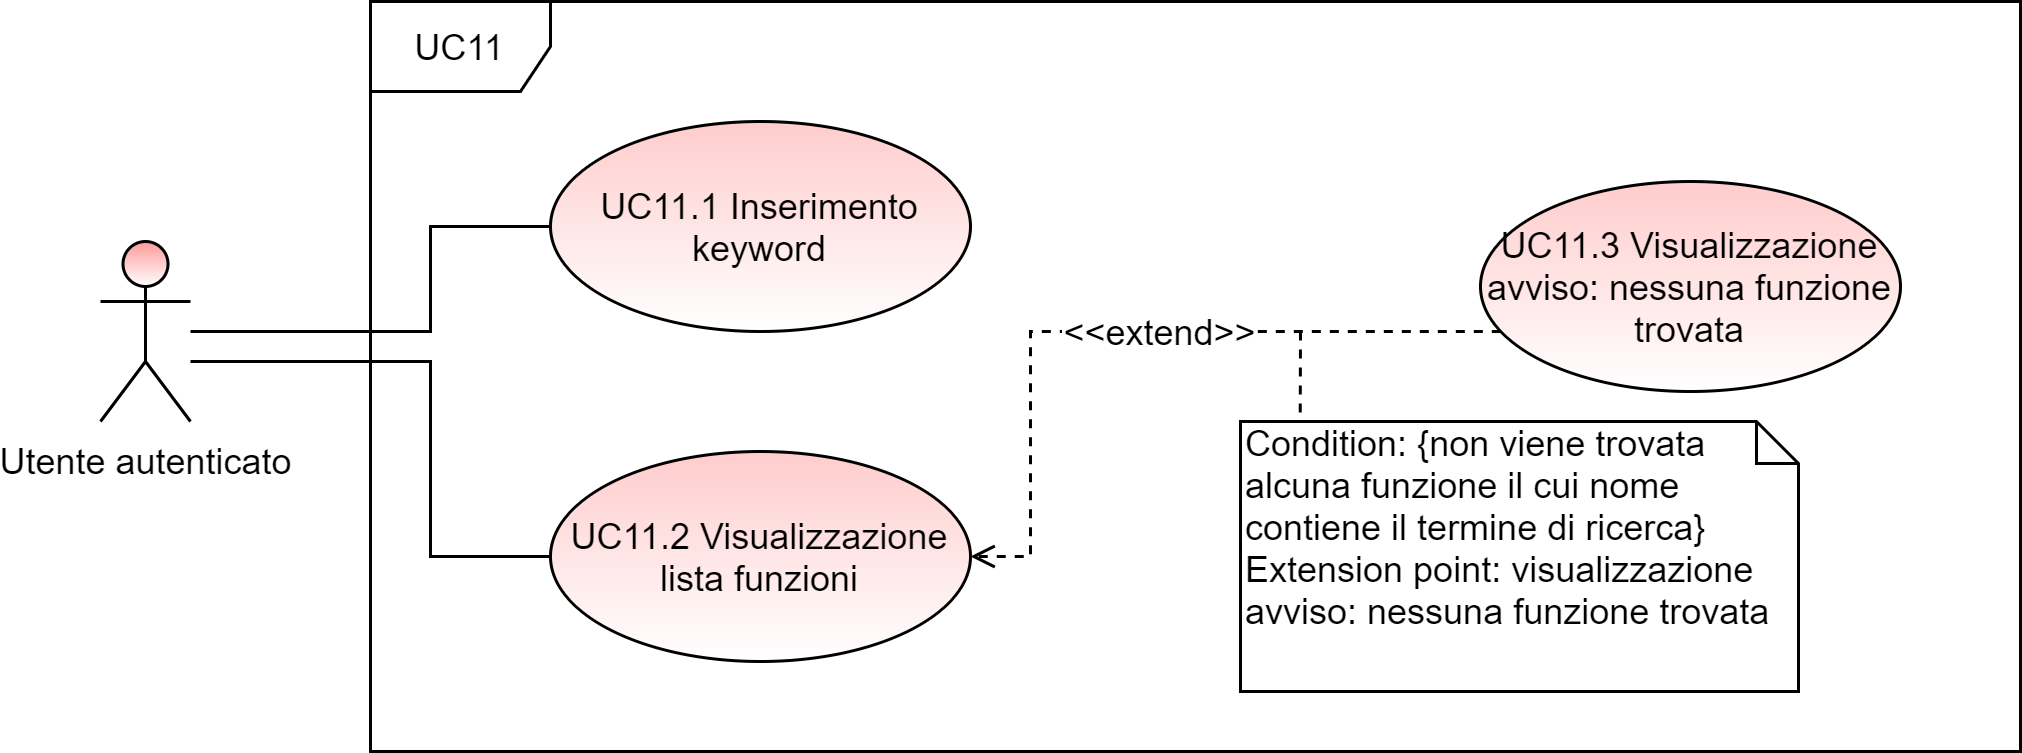
\includegraphics[scale=\ucs]{./res/img/UC11.png}
	\caption {UC11 - Ricerca funzione per nome}
\end{figure}
\begin{itemize}
	\item \textbf{Attori primari:} \ua{};
	\item \textbf{Attori secondari:} \re{};
	\item \textbf{Descrizione:} l’utente richiede la visualizzazione della lista di tutte le funzioni il cui nome contiene un certo termine di ricerca eseguendo il comando \psearch{}. Il sistema riporta la lista di tali funzioni;
	\item \textbf{Scenario principale:} 
	\begin{itemize}
		\item l’utente inserisce correttamente ed esegue il comando \psearch{};
		\item il sistema stampa la lista di tutte le funzioni il cui nome contiene il termine di ricerca.
	\end{itemize}
	\item \textbf{Precondizione:} l’utente desidera individuare tutte le funzioni correlate ad un certo termine;
	\item \textbf{Postcondizione:} la CLI\ped{\textit{G}} riporta la lista di tutte le funzioni il cui nome contiene il termine di ricerca specificato nel comando \search{}.
\end{itemize}